\documentclass[9pt]{article}

%l'espace interligne
\usepackage{setspace}
%les images
\usepackage{graphicx}
	\graphicspath{ {../} }
 %tableaux multipages
\usepackage{longtable}
%pour gerer les flotant -> images
\usepackage{float}
%séparer la page en 2
\usepackage{blindtext}
%tableaux pour les bytefields
\usepackage{bytefield}
%tableaux à pleins de colones
\usepackage{multicol}
% avoir des tableaux et des images propres en multicols
\usepackage{wrapfig}
%theorical computer science symbols
\usepackage{stmaryrd}
%little lines on the tables
\usepackage{booktabs}
%ajoute les slash dans les tables
\usepackage{diagbox}
%indent after a section title
\usepackage{indentfirst}
%use of boxes ... encadrer du text
\usepackage{awesomebox}
%ajout des emojis
\usepackage{emoji}
%maths symbols
\usepackage{amssymb}
\usepackage{amsmath}
	\newcommand{\Lapl}{\mathop{\mathcal{L}}}
\usepackage{mathtools}
    \DeclarePairedDelimiter\floor{\lfloor}{\rfloor}
%avoir du UTF8
\usepackage[utf8]{inputenc}
	\pagenumbering{arabic}
%police francais
\usepackage[T1]{fontenc}
%Avoir Tables de matiere en fr
\usepackage[french,english]{babel}
%insertion pdf
\usepackage{pdfpages}
%add the refs
\usepackage[style=ieee]{biblatex}
\addbibresource{ref.bib}
%\addbibresource{res.bib}
%couleurs
\usepackage{xcolor}
	\definecolor{codegreen}{rgb}{0,0.6,0}
	\definecolor{codegray}{rgb}{0.5,0.5,0.5}
	\definecolor{codepurple}{rgb}{0.58,0,0.82}
	\definecolor{backcolour}{rgb}{0.95,0.95,0.92}


    \definecolor{mGreen}{rgb}{0,0.6,0}
    \definecolor{mGray}{rgb}{0.5,0.5,0.5}
    \definecolor{mPurple}{rgb}{0.58,0,0.82}
    \definecolor{backgroundColour}{rgb}{0.95,0.95,0.92}

%avoir des listes
\usepackage{listings}
% RISC-V Assembler syntax and style for latex lstlisting package
% 
% These are risc-v commands as per our university (University Augsburg, Germany) guidelines.
%
% Author: Anton Lydike
%
% This code is in the public domain and free of licensing

% language definition
\lstdefinelanguage[RISC-V]{Assembler}
{
  alsoletter={.}, % allow dots in keywords
  alsodigit={0x}, % hex numbers are numbers too!
  morekeywords=[1]{ % instructions
    lb, lh, lw, lbu, lhu,
    sb, sh, sw,
    sll, slli, srl, srli, sra, srai,
    add, addi, sub, lui, auipc,
    xor, xori, or, ori, and, andi,
    slt, slti, sltu, sltiu,
    beq, bne, blt, bge, bltu, bgeu,
    j, jr, jal, jalr, ret,
    scall, break, nop
  },
  morekeywords=[2]{ % sections of our code and other directives
    .align, .ascii, .asciiz, .byte, .data, .double, .extern,
    .float, .globl, .half, .kdata, .ktext, .set, .space, .text, .word
  },
  morekeywords=[3]{ % registers
    zero, ra, sp, gp, tp, s0, fp,
    t0, t1, t2, t3, t4, t5, t6,
    s1, s2, s3, s4, s5, s6, s7, s8, s9, s10, s11,
    a0, a1, a2, a3, a4, a5, a6, a7,
    ft0, ft1, ft2, ft3, ft4, ft5, ft6, ft7,
    fs0, fs1, fs2, fs3, fs4, fs5, fs6, fs7, fs8, fs9, fs10, fs11,
    fa0, fa1, fa2, fa3, fa4, fa5, fa6, fa7
  },
  morecomment=[l]{;},   % mark ; as line comment start
  morecomment=[l]{\#},  % as well as # (even though it is unconventional)
  morestring=[b]",      % mark " as string start/end
  morestring=[b]'       % also mark ' as string start/end
}

% usage example:

% define some basic colors
\definecolor{mauve}{rgb}{0.58,0,0.82}

\lstdefinestyle{riscv}{
    language=[RISC-V]{Assembler}, 
    backgroundcolor=\color{white}, 
    numberstyle=\tiny\color{codegray},
    stringstyle=\color{white},
    basicstyle=\footnotesize\sffamily\color{black},
    breakatwhitespace=false,         
    breaklines=true, 
    rulecolor=\color{black},
    captionpos=b,                    
    keepspaces=true,                 
    numbers=none,                    
    numbersep=5pt,                  
    showspaces=false,                
    showstringspaces=false,
    showtabs=false,                  
    tabsize=2,
    escapeinside={<@}{@>}
}

\lstdefinestyle{console}{
        backgroundcolor=\color{black}, 
        numberstyle=\tiny\color{codegray},
        stringstyle=\color{white},
        basicstyle=\tiny\sffamily\color{white},
        breakatwhitespace=false,         
        breaklines=true, 
        rulecolor=\color{black},
        captionpos=b,                    
        keepspaces=true,                 
        numbers=none,                    
        numbersep=5pt,                  
        showspaces=false,                
        showstringspaces=false,
        showtabs=false,                  
        tabsize=2
    }
\lstdefinestyle{consoleLarge}{
    backgroundcolor=\color{black}, 
    numberstyle=\tiny\color{codegray},
    stringstyle=\color{white},
    basicstyle=\footnotesize\sffamily\color{white},
    breakatwhitespace=false,         
    breaklines=true, 
    rulecolor=\color{black},
    captionpos=b,                    
    keepspaces=true,                 
    numbers=none,                    
    numbersep=5pt,                  
    showspaces=false,                
    showstringspaces=false,
    showtabs=false,                  
    tabsize=2
}
    
%liens/references	
\usepackage{hyperref}
	\hypersetup{
    		colorlinks=true,
    		linkcolor=blue,
    		filecolor=magenta,
    		urlcolor=cyan,
	}
%captions -> descriptions d'elements
\usepackage{caption}
\usepackage{subcaption}
%tableaux
\usepackage{array,multirow,makecell}
	\setcellgapes{1pt}
	\makegapedcells
	\newcolumntype{R}[1]{>{\centering\arraybackslash }b{#1}}
	\newcolumntype{L}[1]{>{\centering\arraybackslash }b{#1}}
	\newcolumntype{C}[1]{>{\centering\arraybackslash }b{#1}}
%lipsum pour faire du template
\usepackage{lipsum}
%les marges et formats de pages
\usepackage{geometry}
 	\geometry{a4paper,
 			total={170mm,257mm},
 			left=20mm,
 			top=20mm,}
%s'assurer qu'on a bien les section en roman
\renewcommand{\thesection}{\Roman{section}}
\renewcommand{\thesubsection}{\thesection.\Roman{subsection}}
%fonction pour faire une division de la page en 3 horizontales
\newcommand\textline[4][t]{%
  \par\smallskip\noindent\parbox[#1]{.5\textwidth}{\raggedright#2}%
  \parbox[#1]{.5\textwidth}{\raggedleft{#3}}\par\smallskip%
}

\makeatletter
  \renewcommand\l@section{\@dottedtocline{2}{1.5em}{3em}}
  \renewcommand\l@subsection{\@dottedtocline{2}{3em}{5em}}
  \renewcommand\l@subsubsection{\@dottedtocline{2}{6em}{7em}}
\makeatother

\usepackage[newfloat]{minted}
\newenvironment{code}{\captionsetup{type=listing}}{}
\SetupFloatingEnvironment{listing}{name=Source Code}
%schémas 
\usepackage{tikz}
\usetikzlibrary{positioning,shapes,shadows,arrows,intersections}
\usetikzlibrary{positioning}
\usetikzlibrary{decorations.text}
\usetikzlibrary{decorations.pathmorphing}
\usepackage{pgfplots}
\usepackage{circuitikz}
%\tikzstyle{arduidev}=[draw, text width=6em, minimum height=8em]


\singlespacing

\begin{document}
\begin{titlepage}

\begin{figure}[ht]
    \centering
    
\includegraphics[width=10cm]{img/logo_partenairs.png}
\end{figure}
\begin{center}
	\noindent\rule{9cm}{0.4pt}

	\begin{spacing}{2}


	{\huge\bfseries "Les Vieux bRISCards" final report from 
\includegraphics[width=3cm]{img/logoCentrale.png} \textbf{Rennes}} \\
	{\large  3rd national RISC-V student contest - 2022-2023}
	\end{spacing}

	\noindent\rule{8cm}{0.4pt}
\end{center}

	\begin{spacing}{1}
	{\large \textbf{Authors :} }\hfill{\large \textbf{Professor :} }\\
	{Majed Abdennadher}\hfill{Guillaume Hiet}\\
    {Thomas Chevalier}\hfill{Rubén Salvador}\\
    {Ulysse Vincenti}
	\end{spacing}
\begin{center}
	\tableofcontents

\vspace*{\fill}

\end{center}

\begin{flushright}
	Rennes, \today
\end{flushright}

\end{titlepage}

\clearpage 



\paragraph{Abstract :}

The 5\textsuperscript{rd} national RISC-V student contest is a hackaton sponsored by Thales, the GDR SOC\textsuperscript{2} and the CNFM whose goal is to improve the security of the CV32A6 RISC-V soft-core. The task is to defeat ten memory-corruption attacks taken from the RIPE benchmark with minimal performance overhead. The soft-core is geared with Zephyr RTOS, and the contest allows us to modify the CV32A6 core, the OS and/or the compiler. Our solution consists of a forward edge control-flow integrity (FW-CFI) enforcement technique, a shadow stack and a hardened version of memset that protects against heap pointer read or write overflow. Our implementation modifies the CV32A6 core in order to add support for hardware CFI checks and the shadow stack. We also modify the compiler for automatic generation of CFI annotations, as well as the OS and the linked libraries.

The objective of this challenge is to counter a maximum number of attacks in a batch of 10 attacks from the RIPE benchmark ported to RISC-V CVA6-32. 
Numerous of theses attacks are ways to take control of the control flow. 
With the control of the flow, the attacker can realise \textbf{arbitrary code execution}. It is therefore, of the greatest importance to keep the control of the flow.
Multiple countermeasure exist for theses attacks and we based our solution on one of them : \textit{Intel Control-flow Enforcement}\cite{intel_cet} (CFE).

Our solution, is a forward edge control-flow integrity (FW-CFI) enforcement technic, a shadow stack(SS) and a memset heap protection. We have tested multiple solution before going for this one. With this implementation we are able to \textbf{counter all the attacks given} with no apparent timing overhead.

\vspace{1cm}

\begin{multicols}{2}

\section{Introduction}
The national RISC-V student contest is open to all Master 2 students of a French engineering school or University. 
Each team can count up to 4 members and can be coached by teachers or PhD students. 
For the last 3 years, this contest has proposed hardware challenges to the students, the first year was focused on the FPGA optimisation of the core, the second year on the power efficiency and finally this year pays attention to the security of the core. 
A benchmark of 10 attacks is given to the participants, the goal is to prevent the attacks on a Zephyr running upon the CV32A6. 
The chosen board is a Zybo-z7 20 which embeds an Artix-7 FPGA. 
The implementation should not increase the size of the FPGA design or the execution time by more than 100\%. 
The teams are judged on the number of attacks they are able to counter and in the case of a tie, on the execution time of a performance benchmark.




\paragraph{The core} CV32A6 is an open source 6 stage RISC-V 32 bit processor. It implements I, M and C extensions from the RISC-V instruction set \cite{riscv_isa}. The goal of this core is to run an OS at reasonable speed. The chosen core does not have a MMU or PMP but theses features are available on more recent version of the core. 

\begin{figure}[H]
    \centering
    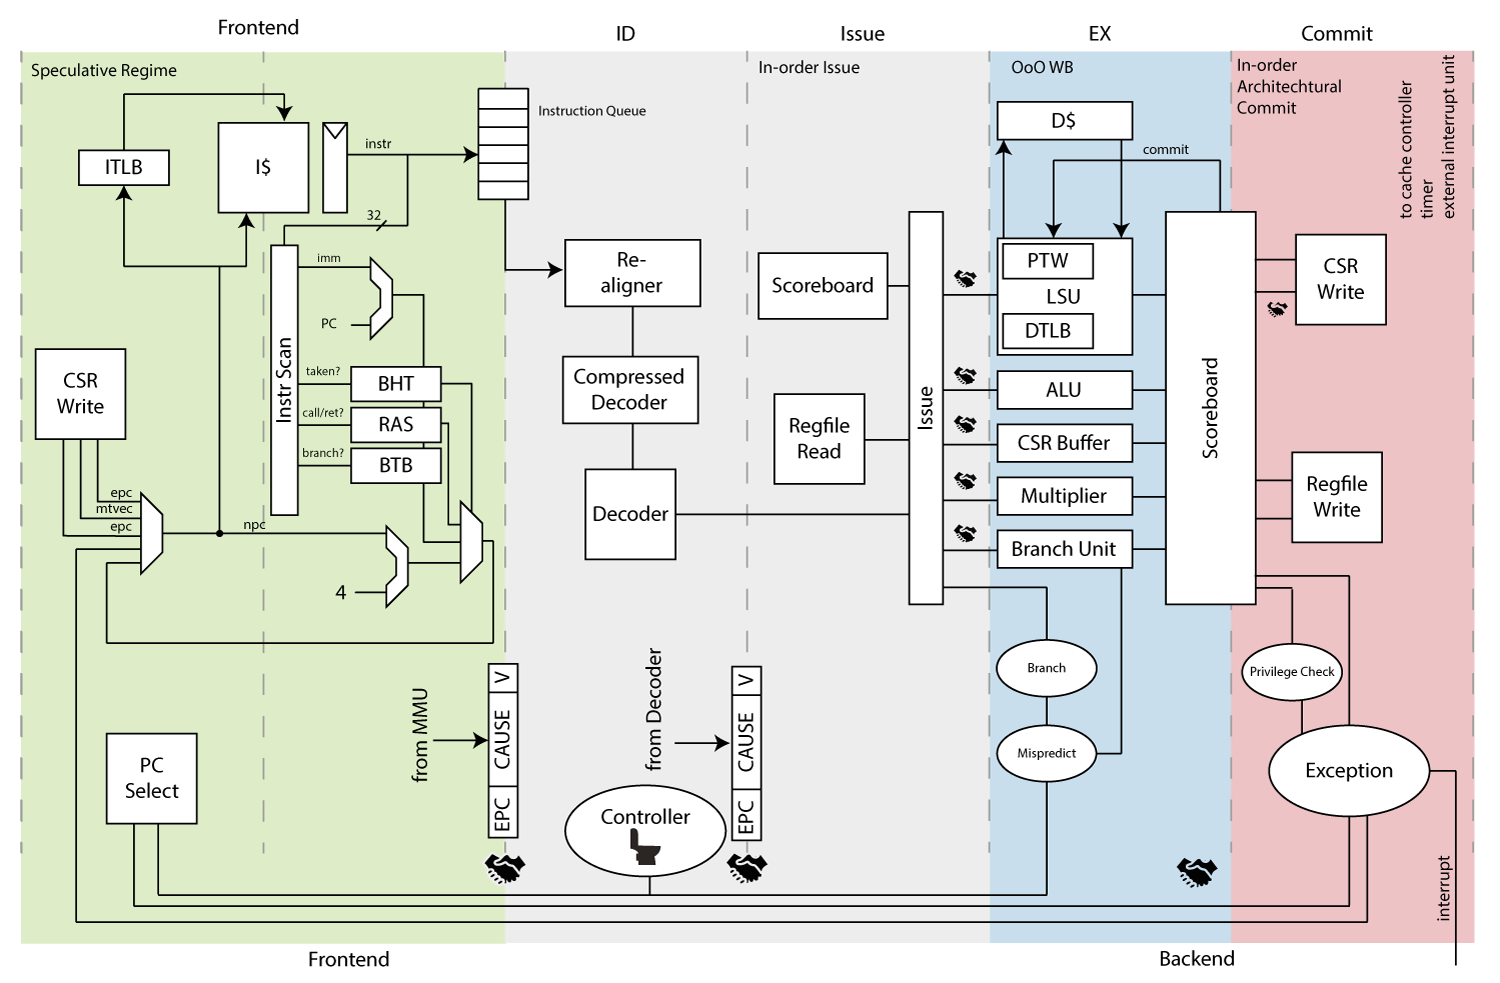
\includegraphics[width=0.4\linewidth]{img/core_diagram.png}
    \caption{CVA6 core diagram \cite{cva6_doc}}
    \label{fig:core_diag}
\end{figure}

\paragraph{Zephyr} is an embedded real-time OS which supports a wide variety of microprocessor/microcontrollers architectures.
Zephyr embeds multiple services and features like PMP support, single address space and stack canaries. 
The OS uses Kconfig and device tree for its configuration and is compiled through cmake with gcc-12.   

\paragraph{Runtime Intrusion Prevention Evaluator (Ripe) \cite{ripe_attack}} is a security benchark which contains 850 executable simulated attacks. The goal of this bench is to evaluate solutions against buffer overflows attacks. The benchmark was recently ported to RISC-V and a selection of 10 of theses attacks makes our evaluation benchmark.
% ret2libc simulation is not done to libc but with a defined function in the ripe program and the rop simulation is done without gadgets and no offset is used in the indirect call for the rop attack.


\begin{wraptable}{l}{0.7\linewidth}
\centering
    \centering
    \tiny
    \begin{tabular}{c||c|c|c|c|c}
         i & approaches & inject param & code ptr & location & function \\ \hline \hline
         1 & direct & no nop & ret  & stack & memcpy\\\hline
         2 & direct & no nop & functptrstackvar & stack & memcpy\\\hline
         3 & indirect & no nop & functptrstackvar & stack & memcpy\\\hline
         4 & direct & data & var leak & heap & sprintf\\\hline
         5 & direct & ret2libc& ret & stack & memcpy\\\hline
         6 & indirect & ret2libc & funcptrheapvar & heap & memcpy\\\hline
         7 & indirect & ret2libc & structfunctptrheap & heap & homebrew\\\hline
         8 & indirect & ret2libc & longjumpbugheap&heap&memcpy\\\hline
         9 & direct & rop & ret&stack&memcpy\\\hline
         10& direct & rop & structfuncptrheap&heap&memcpy\\
    \end{tabular}
     \makeatletter\def\@captype{table}\makeatother
    \caption{Table presenting the different supposedly simulated attacks on the benchmark}
\end{wraptable}

\subsection{Related work}
Multiple methods exist for the control flow enforcement. 
% faire une partie sur le papier de RIPE
% faire partie sur le Intel CFE

The RIPE (Runtime Intrusion Prevention Evaluator) is a testbed which cover 850 forms of buffer overflows. To do so it 

Some of the first ideas that could come to mind would be ASLR. However, this solution is sub optimal because the chosen core is 32 bits. As a side note, the RIPE benchmark takes the form of a single binary that attacks itself and thus defeat any countermeasures that relies on the secrecy of memory locations. 


% partie sur le fait qu'en réalité les attaques sont assez mal simulé.


\section{Implementation}

\subsection{Stack canaries}
The stack canaries are a simple tool to implement with Zephyr because it only demands to add 2 lines in the configuration file of the board. Stack canaries are secret pseudo random value placed on the stack to check the integrity of this memory space. If stack smashing occurs, the canary might be overwritten and the smashing detected.

\begin{lstlisting}
    CONFIG_TEST_RANDOM_GENERATOR=y
    CONFIG_STACK_CANARIES=y
\end{lstlisting}
The first line is here to add a pseudo random source and the second one is to add the stack canary. 

\subsection{Simple FW \& BW control flow}

The development of forward edge and backward edge control flow enforcement has been thought of with 2 custom instructions : the first one as a landing pad (LP) after a call : "\textit{li zero, 2}", this is the forward edge control flow. The second instruction is the LP which would be placed after a call so that when the call returns, the first instruction executed is this instruction : "\textit{li zero, 1}". 

The result in assembly is : 

\lstinputlisting[caption={Example of "z\_bss\_zero" function compiled with the pads}, style={riscv}]{listings/z_bss_zero_1.asm}

The instruction "nop" is in reality : "\textit{add zero, 0}", that is why we chose the solution of the index 1 and 2.
This technique has been quite efficient. Added to the stack canaries we were able to break :

% place attacks counterfeited through the simple landing pad technique

\tikzstyle{inst} = [rectangle, draw, fill=white, text centered, draw=black, minimum width=2.5cm, minimum height=.4cm]
\tikzstyle{arrow} = [thick,->,>=stealth]

\begin{figure}[H]
\centering
\begin{circuitikz}[node distance=.4cm]


\node (inst3) [inst] {...};
\node (inst5) [inst, below of=inst3] {\tiny jalr  a5};

\node (inst6) [inst, below of=inst5, xshift=3cm] {\tiny li zero, 2};
\node (inst7) [inst, below of=inst6] {\tiny ...};
\node (inst8) [inst, below of=inst7] {\tiny ret};

\node (inst9) [inst, below of=inst8, xshift=-3cm] {\tiny li, zero, 1};
\node (inst10) [inst, below of=inst9] {\tiny ...};



% ---------------

\draw [arrow] (inst5.south east) -- (inst6.north west);

%\draw [decoration={text along path,
%        text={ss.push(PC + 4)},text align={center}}, decorate, yshift=0.3cm] (inst5.south east) -- (inst6.north west);


\draw [arrow] (inst8.south west) -- (inst9.north east);
%\draw [decoration={text along path,
%        text={ss.pop()},text align={center}}, decorate, yshift=0.3cm] (inst9.north east) -- (inst8.south west);

\end{circuitikz}
\caption{Control Flow Diagram : simple implementation}
\end{figure}



In a second time, we thought about identifying the function where indirect calls could go. This was achieved by adding some information in the first LP. 
The first 2 bits of the immediate was kept as it was.  The last bit was taken by isVariadic information and the rest of the immediate became the number of arguments. 



\vspace{1em}

\begin{figure}[H]
\centering
\begin{bytefield}[bitwidth=1.1em]{32}
    \bitheader{0-31} \\
    \bitbox{1}{V} & \bitbox{8}{number args} & \bitbox{1}{1}& \bitbox{1}{0}
    & \bitbox{21}{nop} \\
\end{bytefield}
\caption{Landing Pad for the FW-CFI}
\end{figure}

\begin{itemize}
    \item V : the variadic bit. 
\end{itemize}

But, to check whether or not the call is made with the right number of arguments, the hardware must be aware of this information, this is done by writing this information to a custom CSR.

\tikzstyle{inst} = [rectangle, draw, fill=white, text centered, draw=black, minimum width=2.5cm, minimum height=.4cm]
\tikzstyle{arrow} = [thick,->,>=stealth]

\begin{figure}[H]
\centering
\begin{circuitikz}[node distance=.4cm]


\node (inst3) [inst] {...};
\node (inst4) [inst, below of=inst3] {\tiny csrwi CSTM\_CSR, 1 };
\node (inst5) [inst, below of=inst4] {\tiny jalr  a5};

\node (inst6) [inst, below of=inst5, xshift=3cm] {\tiny li zero, 6};
\node (inst7) [inst, below of=inst6] {\tiny ...};
\node (inst8) [inst, below of=inst7] {\tiny ret};

\node (inst9) [inst, below of=inst8, xshift=-3cm] {\tiny li, zero, 1};
\node (inst10) [inst, below of=inst9] {\tiny ...};



% ---------------

\draw [arrow] (inst5.south east) -- (inst6.north west);

%\draw [decoration={text along path,
%        text={ss.push(PC + 4)},text align={center}}, decorate, yshift=0.3cm] (inst5.south east) -- (inst6.north west);


\draw [arrow] (inst8.south west) -- (inst9.north east);
%\draw [decoration={text along path,
%        text={ss.pop()},text align={center}}, decorate, yshift=0.3cm] (inst9.north east) -- (inst8.south west);

\end{circuitikz}
\caption{Control Flow Diagram : indirect call}
\end{figure}



\subsection{Forward CFI + Shadow Stack}

\tikzstyle{inst} = [rectangle, draw, fill=white, text centered, draw=black, minimum width=2.5cm, minimum height=.4cm]
\tikzstyle{arrow} = [thick,->,>=stealth]

\begin{figure}[H]
\centering
\begin{circuitikz}[node distance=.4cm]


\node (inst3) [inst] {\tiny ...};
\node (inst4) [inst, below of=inst3] {\tiny csrwi CSTM\_CSR, 1 };
\node (inst5) [inst, below of=inst4] {\tiny jalr  a5};

\node (inst6) [inst, below of=inst5, xshift=5cm] {\tiny li zero, 6};
\node (inst7) [inst, below of=inst6] {\tiny ...};
\node (inst8) [inst, below of=inst7] {\tiny ret};

\node (inst9) [inst, below of=inst8, xshift=-5cm] {\tiny ...};



% ---------------

\draw [arrow] (inst5.south east) -- (inst6.north west);

\draw [decoration={text along path,
        text={|\tiny|ss.push(PC + 4)},text align={center}, raise=1mm}, decorate] (inst5.south east) -- (inst6.north west);


\draw [arrow] (inst8.south west) -- (inst9.north east);
\draw [decoration={text along path,
        text={|\tiny|ss.pop()},text align={center}, raise=1mm}, decorate] (inst9.north east) -- (inst8.south west);

\end{circuitikz}
\caption{Control Flow Diagram : indirect call with shadow stack}
\end{figure}


The shadow stack allows to remove the second LP. A shadow stack is a hardware or software security feature which stores the return addresses of a call in a LIFO secured space. During a return, the return address is checked against the shadow stack return address. If the return address in the shadow stack and the return address in the current flow are not the same, their might be an attack occurring.

\tikzstyle{io} = [trapezium, trapezium left angle=70, trapezium right angle=110, minimum width=2cm, minimum height=.5cm, text centered, draw=black]
\tikzstyle{process} = [rectangle, minimum width=2cm, minimum height=.5cm, text centered, draw=black]
\tikzstyle{decision} = [diamond, draw, text badly centered, inner sep=3pt, aspect=3]
\tikzstyle{line_meeting} = [circle, draw, fill=black]

 \tikzstyle{every node}=[font=\small]

\tikzstyle{line} = [thick]
\tikzstyle{arrow} = [thick,->,>=stealth]
\tikzstyle{startstop} = [rectangle, rounded corners, minimum width=2cm, minimum height=1cm,text centered, draw=black]

\begin{figure}[H]
\centering
\begin{circuitikz}[node distance=1cm]

\node (start) [startstop] {Start};
\node (in1) [io, below of=start] {new inst};

\node (dec1) [decision, below of=in1] {is CALL ?};
\node (pro1) [process, below of=dec1] {set NEXT\_INST\_LP};
\node (pro2) [process, below of=pro1] {SS.push(PC + 4)};

\node (start2) [startstop,right of=start, xshift=2.5cm] {Start};
\node (in2) [io, below of=start2] {new inst};
\node (dec2) [decision, below of=in2] {is RET ?};
\node (dec4) [decision, below of=dec2, yshift=-.5cm] {PC!=SS.pop()};

\node (start3) [startstop,right of=start2, xshift=4.5cm] {Start};
\node (in3) [io, below of=start3] {new inst};

\node (dec5) [decision, below of=in3, yshift=-0.5cm] {is NEXT\_INST\_LP set ?};
\node (dec3) [decision, below of=dec5, yshift=-0.5cm] {is LP ?};
\node (dec7) [decision, below of=dec3, xshift=-2cm, yshift=-0.5cm] {LP.VARIADIC ?};
\node (dec6) [decision, below of=dec7,yshift=-1cm] {\tiny LP.ARGS\_NB <= CSR.ARGS\_NB};
\node (dec8) [decision, right of=dec7, yshift=-1cm, xshift=3cm] {\tiny LP.ARGS\_NB == CSR.ARGS\_NB};
\node (pro3) [process, below of=dec3, yshift=-4.5cm] {unset NEXT\_INST\_LP};


\node (stop) [startstop, below of=dec4, yshift=-5cm] {Exception};
% \node (pro2b) [process, right of=dec1, xshift=2cm] {Process 2b};


% ''''''''''''''''
\draw [arrow] (start) -- (in1);
\draw [arrow] (in1) -- (dec1);

\draw [arrow] (dec1.south) -- (pro1.north);
\draw [arrow] (pro1.south) -- (pro2.north);

\draw [arrow] (dec1.west) -- (-2.5, -2) -- (-2.5, 0) -- (start);
\draw [line](pro2.south) -- (0, -5) -- (-2.5, -5) -- (-2.5, -2) node[line_meeting]{};

% ----------------
\draw [arrow] (start2) -- (in2);
\draw [arrow] (in2) -- (dec2);


\draw [arrow] (dec2.east) -- (5.7,-2) -- (5.7,0) -- (start2);
\draw [line](dec4.east) -- (5.7,-3.5) --(5.7,-2) node[line_meeting]{};

\draw [arrow] (dec2.south) -- (dec4.north);

\draw [arrow] (dec4) -- (stop);

% ---------------
\draw [arrow] (start3) -- (in3);
\draw [arrow] (in3) -- (dec5);

\draw [arrow] (dec5.south) -- (dec3.north);

\draw [arrow] (dec3.south) -- (9,-4.5) -- (7,-4.5) -- (dec7.north);

\draw [line](dec6.south) -- (7, -8.5) -- (9, -8.5) node[line_meeting]{};

\draw [arrow] (dec7.east) -- (11,-5.5) -- (dec8.north);
\draw [arrow] (dec8.south) -- (11, -8.5) -- (9, -8.5) -- (pro3.north);

\draw [line, name path=ab, arrow] (dec7.south) -- (dec6.north);
\draw[line, name path=cd] (dec8.west) --  (3.5, -6.5) node[line_meeting]{};

%\path[name intersections={of=ab and cd,by=e}];
%\fill[color=white] (e) circle[radius=0.1];
%\draw (e) node[jump crossing]{};


\draw  [line] (dec3.west) --  (5, -4) --  (5, -5) -- (3.5, -5) node[line_meeting]{};

\draw [line](dec6.west) -- (3.5, -7.5) node[line_meeting]{};

\draw [line](dec5.east) -- (14,-2.5) node[line_meeting]{};

\draw [arrow] (pro3.south) --  (9, -10) --  (14, -10) --  (14, 0) -- (start3);



\end{circuitikz}
\caption{Simplified hardware algorithm implemented in the commit stage}
\end{figure}

This scheme was simplified by supposing that their is only one commit per clock cycle done. In reality, we can have up to 2 commits done in one clock cycle, which complexify things. 

The hardware modifications were done with a atypical debug method. For the first half of the competition we did not have access to the simulator. The ILA components did not seem to want to work, therefore, we developed the first elements with the outputs linked to the 9 controllable LEDs of the board. Once the simulator was up and running we did already have a working solution which only needed a verification by the simulator.

To get better results in the FPGA placement, the SS has a depth of only 100. When the count of calls is greater than 100, the SS is deactivated but the previous return addresses are stored. 
The SS starts to compare addresses again when counter goes under 100. 

The previously shown algorithm is implemented through 2 Finite State Machines (FSM) and 2 modules, the first for the detection and FSM, the second for the LIFO logic.

\subsection{Heap "memset" Protection}
%faire des schéma ptetre et des explications des bails 

\subsection{Optimisation}
The first version of the compiled library showed a great lack of optimisation, multiples solutions were applicable to solve that : 
\begin{enumerate}
    \item add an FPU to the core because the performance benchmark is doing floating point operations.
    \item reduce the time consumed by the core on nop execution through prematured nop execution. The custom nop could bypass the pipeline from the fetch phase. Which would remove the timing overhead of the solution.
    \item increase the frequency of the core.
    \item temper the cycle count CSR.
\end{enumerate}

\section{Results}
\subsection{Performances}

\begin{lstlisting}[style=consoleLarge, caption={Results of the benchmark on the non-modified hardware, OS and compiler}]
*** Booting Zephyr OS build zephyr-v3.2.0-327-g869365ab012b  ***
Begining of execution with depth 12, call number 50, seed value 63728127.000000
SUCCESS: computed value 868200.000000 - duration: 25.317176 sec 632929412 cycles
\end{lstlisting}

\begin{lstlisting}[style=consoleLarge, caption={Results of the benchmark on the FW CFI + shadow stack + secure memset HW, OS and compiler}]
*** Booting Zephyr OS build zephyr-v3.2.0-327-g869365ab012b  ***
Begining of execution with depth 12, call number 50, seed value 63728127.000000
SUCCESS: computed value 868200.000000 - duration: 25.135623 sec 628390584 cycles
\end{lstlisting}


\begin{table}[H]
    \centering
    \begin{tabular}{c|c|c}
         & number of cycles & time of execution \\ \hline \hline
         before modifications & 632929412 & 25.317176 sec \\\hline
         stack canaries & 633811376 & 25.352455 sec \\ \hline
         FW \& BW CFI & 628152061 &  25.126082 sec\\ \hline
         FW CFI + shadow stack  & 628152061 &  25.126082 sec \\ \hline
         FW CFI + shadow stack + secure memset & 628390584 &  25.135623  sec
    \end{tabular}
    \caption{Results from the benchmark perf\_baseline before and after the modifications}
\end{table}


\begin{table}[H]
    \centering
    \begin{tabular}{c||c|c}
    resources & utilisation after modification & utilisation before modification \\ \hline\hline
    LUT	& 27161 (51.054512\%) & 25765 (48.43045\%)\\
    FF & 26056 (24.488722\%) & 22328 (20.98\%)\\
    BRAM & 71 (50.714283\%) & 71 (50.714283\%) \\
    clock speed & 25MHz & 25MHz\\
    perf\_baseline size & 86828 B & 61936 B\\
    \end{tabular}
    \caption{Table of modification's impact}
\end{table}

\subsection{Attacks prevented}
\newcolumntype{P}[1]{>{\centering\arraybackslash}p{#1}}
\begin{table}[H]
    \centering
    \begin{tabular}{c|c|P{3cm}|P{2.5cm}|P{2.5cm}}
         index & stack canaries & FW\&BW CFI & FW CFI + shadow stack & FW CFI + shadow stack + secure memset\\ \hline \hline
         1 &    \emoji{check-mark-button} &\emoji{check-mark-button}& \emoji{check-mark-button}& \emoji{check-mark-button}\\\hline
         2 &    \emoji{check-mark-button} &\emoji{check-mark-button}& \emoji{check-mark-button}& \emoji{check-mark-button}\\\hline
         3 &    \emoji{check-mark-button} &\emoji{check-mark-button}& \emoji{check-mark-button}& \emoji{check-mark-button}\\\hline
         4 &    \emoji{cross-mark}        &\emoji{cross-mark}       & \emoji{cross-mark}       & \emoji{check-mark-button}\\\hline
         5 &    \emoji{check-mark-button} &\emoji{check-mark-button} &\emoji{check-mark-button}& \emoji{check-mark-button}\\\hline
         6 &     \emoji{cross-mark}       &\emoji{check-mark-button} &\emoji{check-mark-button}& \emoji{check-mark-button}\\\hline
         7 &     \emoji{cross-mark}       &\emoji{check-mark-button} &\emoji{check-mark-button}& \emoji{check-mark-button}\\\hline
         8 &    \emoji{cross-mark}        &\emoji{check-mark-button} &\emoji{check-mark-button}& \emoji{check-mark-button}\\\hline
         9 &    \emoji{check-mark-button} &\emoji{check-mark-button} &\emoji{check-mark-button}& \emoji{check-mark-button}\\\hline
         10&    \emoji{cross-mark}        &\emoji{check-mark-button} &\emoji{check-mark-button}& \emoji{check-mark-button}\\\hline
    \end{tabular}
    \caption{Table presenting the different prevented attacks with different approaches}
\end{table}


\section{Conclusion}




\section{Annexe}
\begin{centering}
    \begin{longtable}{c c c c}
\begin{minipage}[\baselineskip]{4cm}
 \lstinputlisting[style={console}]{listings/csl_out_1}
\end{minipage}
& 
\begin{minipage}[\baselineskip]{4cm}
  \lstinputlisting[style={console}]{listings/csl_out_2}
\end{minipage}  
& 
\begin{minipage}[\baselineskip]{4cm}
  \lstinputlisting[style={console}]{listings/csl_out_3}
\end{minipage}
&
\begin{minipage}[\baselineskip]{4cm}
  \lstinputlisting[style={console}]{listings/csl_out_4}
\end{minipage}
\\ 1 & 2 & 3 & 4\\ 
\begin{minipage}[\baselineskip]{4cm}
  \lstinputlisting[style={console}]{listings/csl_out_5}
\end{minipage}
 &  
 \begin{minipage}[\baselineskip]{4cm}
\lstinputlisting[style={console}]{listings/csl_out_6}
\end{minipage}
&
  
\begin{minipage}[\baselineskip]{4cm}
\lstinputlisting[style={console}]{listings/csl_out_7}
\end{minipage}
&  

\begin{minipage}[\baselineskip]{4cm}
\lstinputlisting[style={console}]{listings/csl_out_8}
\end{minipage}

\\ 5 & 6 & 7 & 8 \\
&
\begin{minipage}[\baselineskip]{4cm}
\lstinputlisting[style={console}]{listings/csl_out_9}
\end{minipage}
 &
\begin{minipage}[\baselineskip]{4cm}
\lstinputlisting[style={console}]{listings/csl_out_10}
\end{minipage} \\ &  9 & 10 &\\
\caption{Table presenting the different outputs of our solution (suppressing all unprintable characters) }
    \end{longtable}
\end{centering}


\printbibliography

\end{multicols}

\end{document}